\documentclass[12pt]{article}
\usepackage{fullpage,tikz,graphicx}
\graphicspath{./images/}

\title{CS 360: Assignment 1}
\author{Cam J. Loader}

\begin{document}
\maketitle

\begin{enumerate}
  \item Give the state diagrams of the DFAs recognizing the following languages. In all parts the alphabet \sum =\{ 1,0\}:

   \begin{enumerate}
     \item {w $|$ w begins with a 1 and ends with a 0} [4 pts] \\
       \begin{center}
          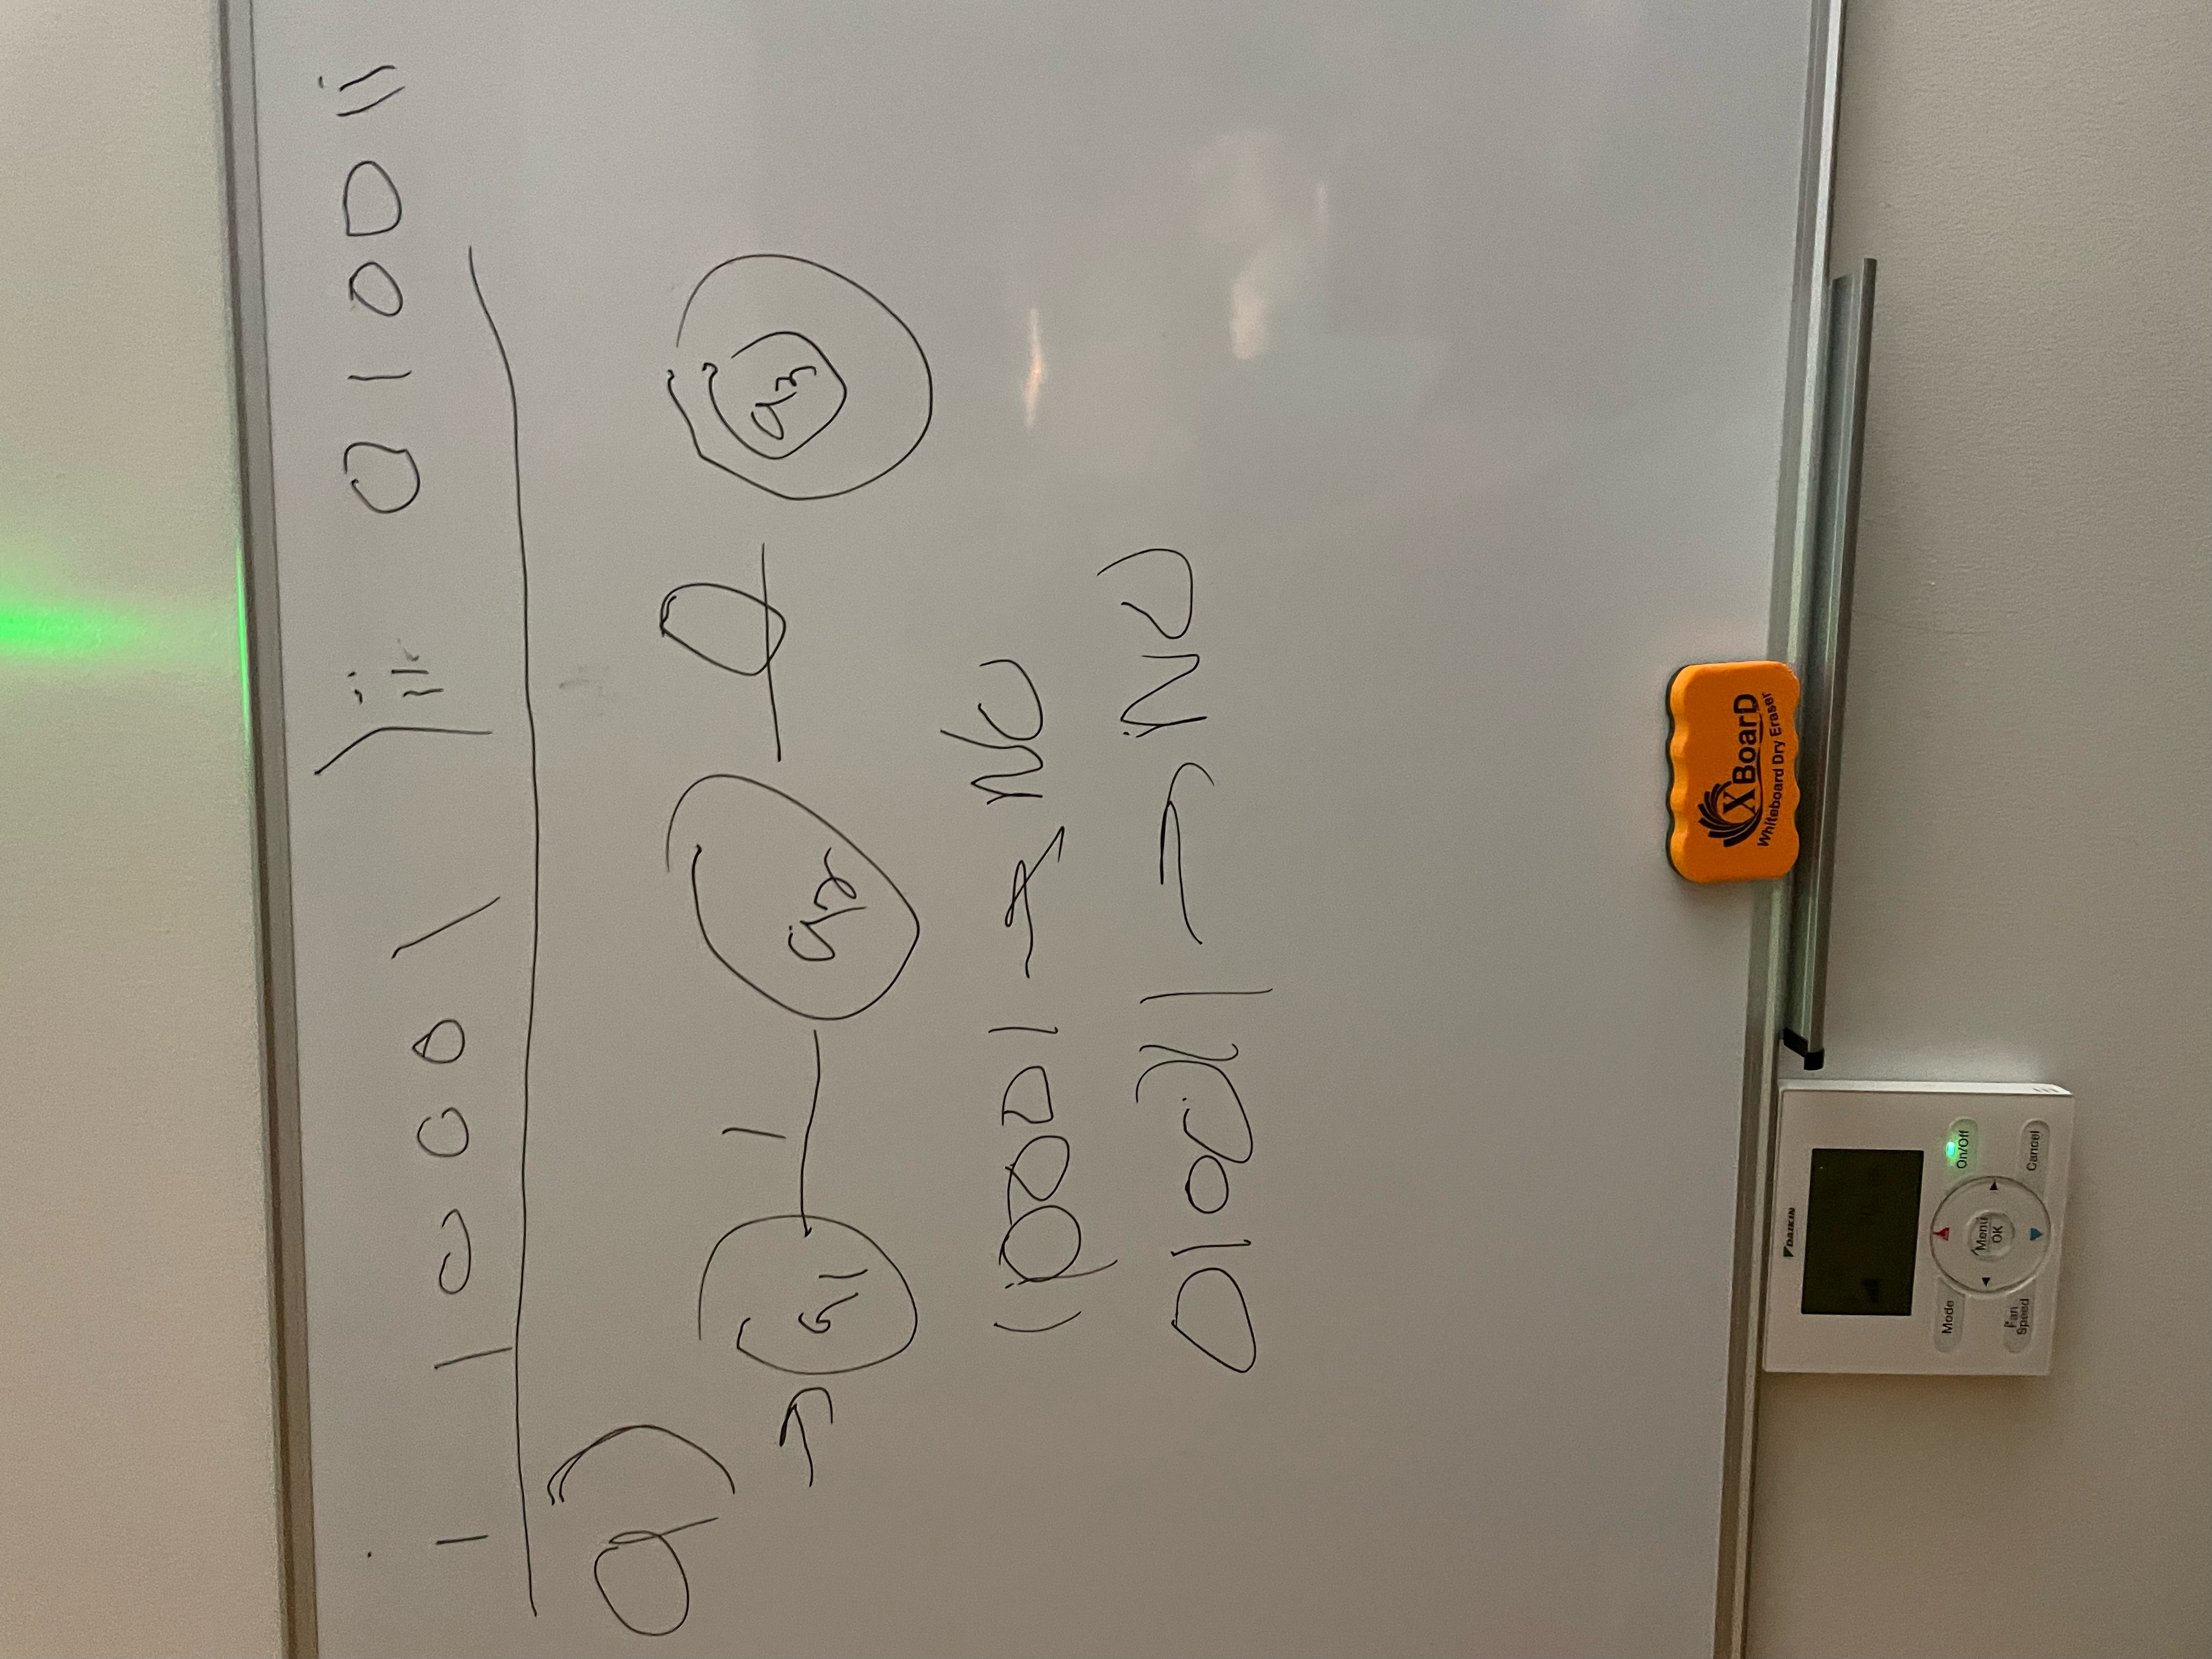
\includegraphics{DFA-a.jpeg}
       \end{center}
     \item item {w $|$ w contains at least three 1s [4 pts] \\
     \begin{center}
          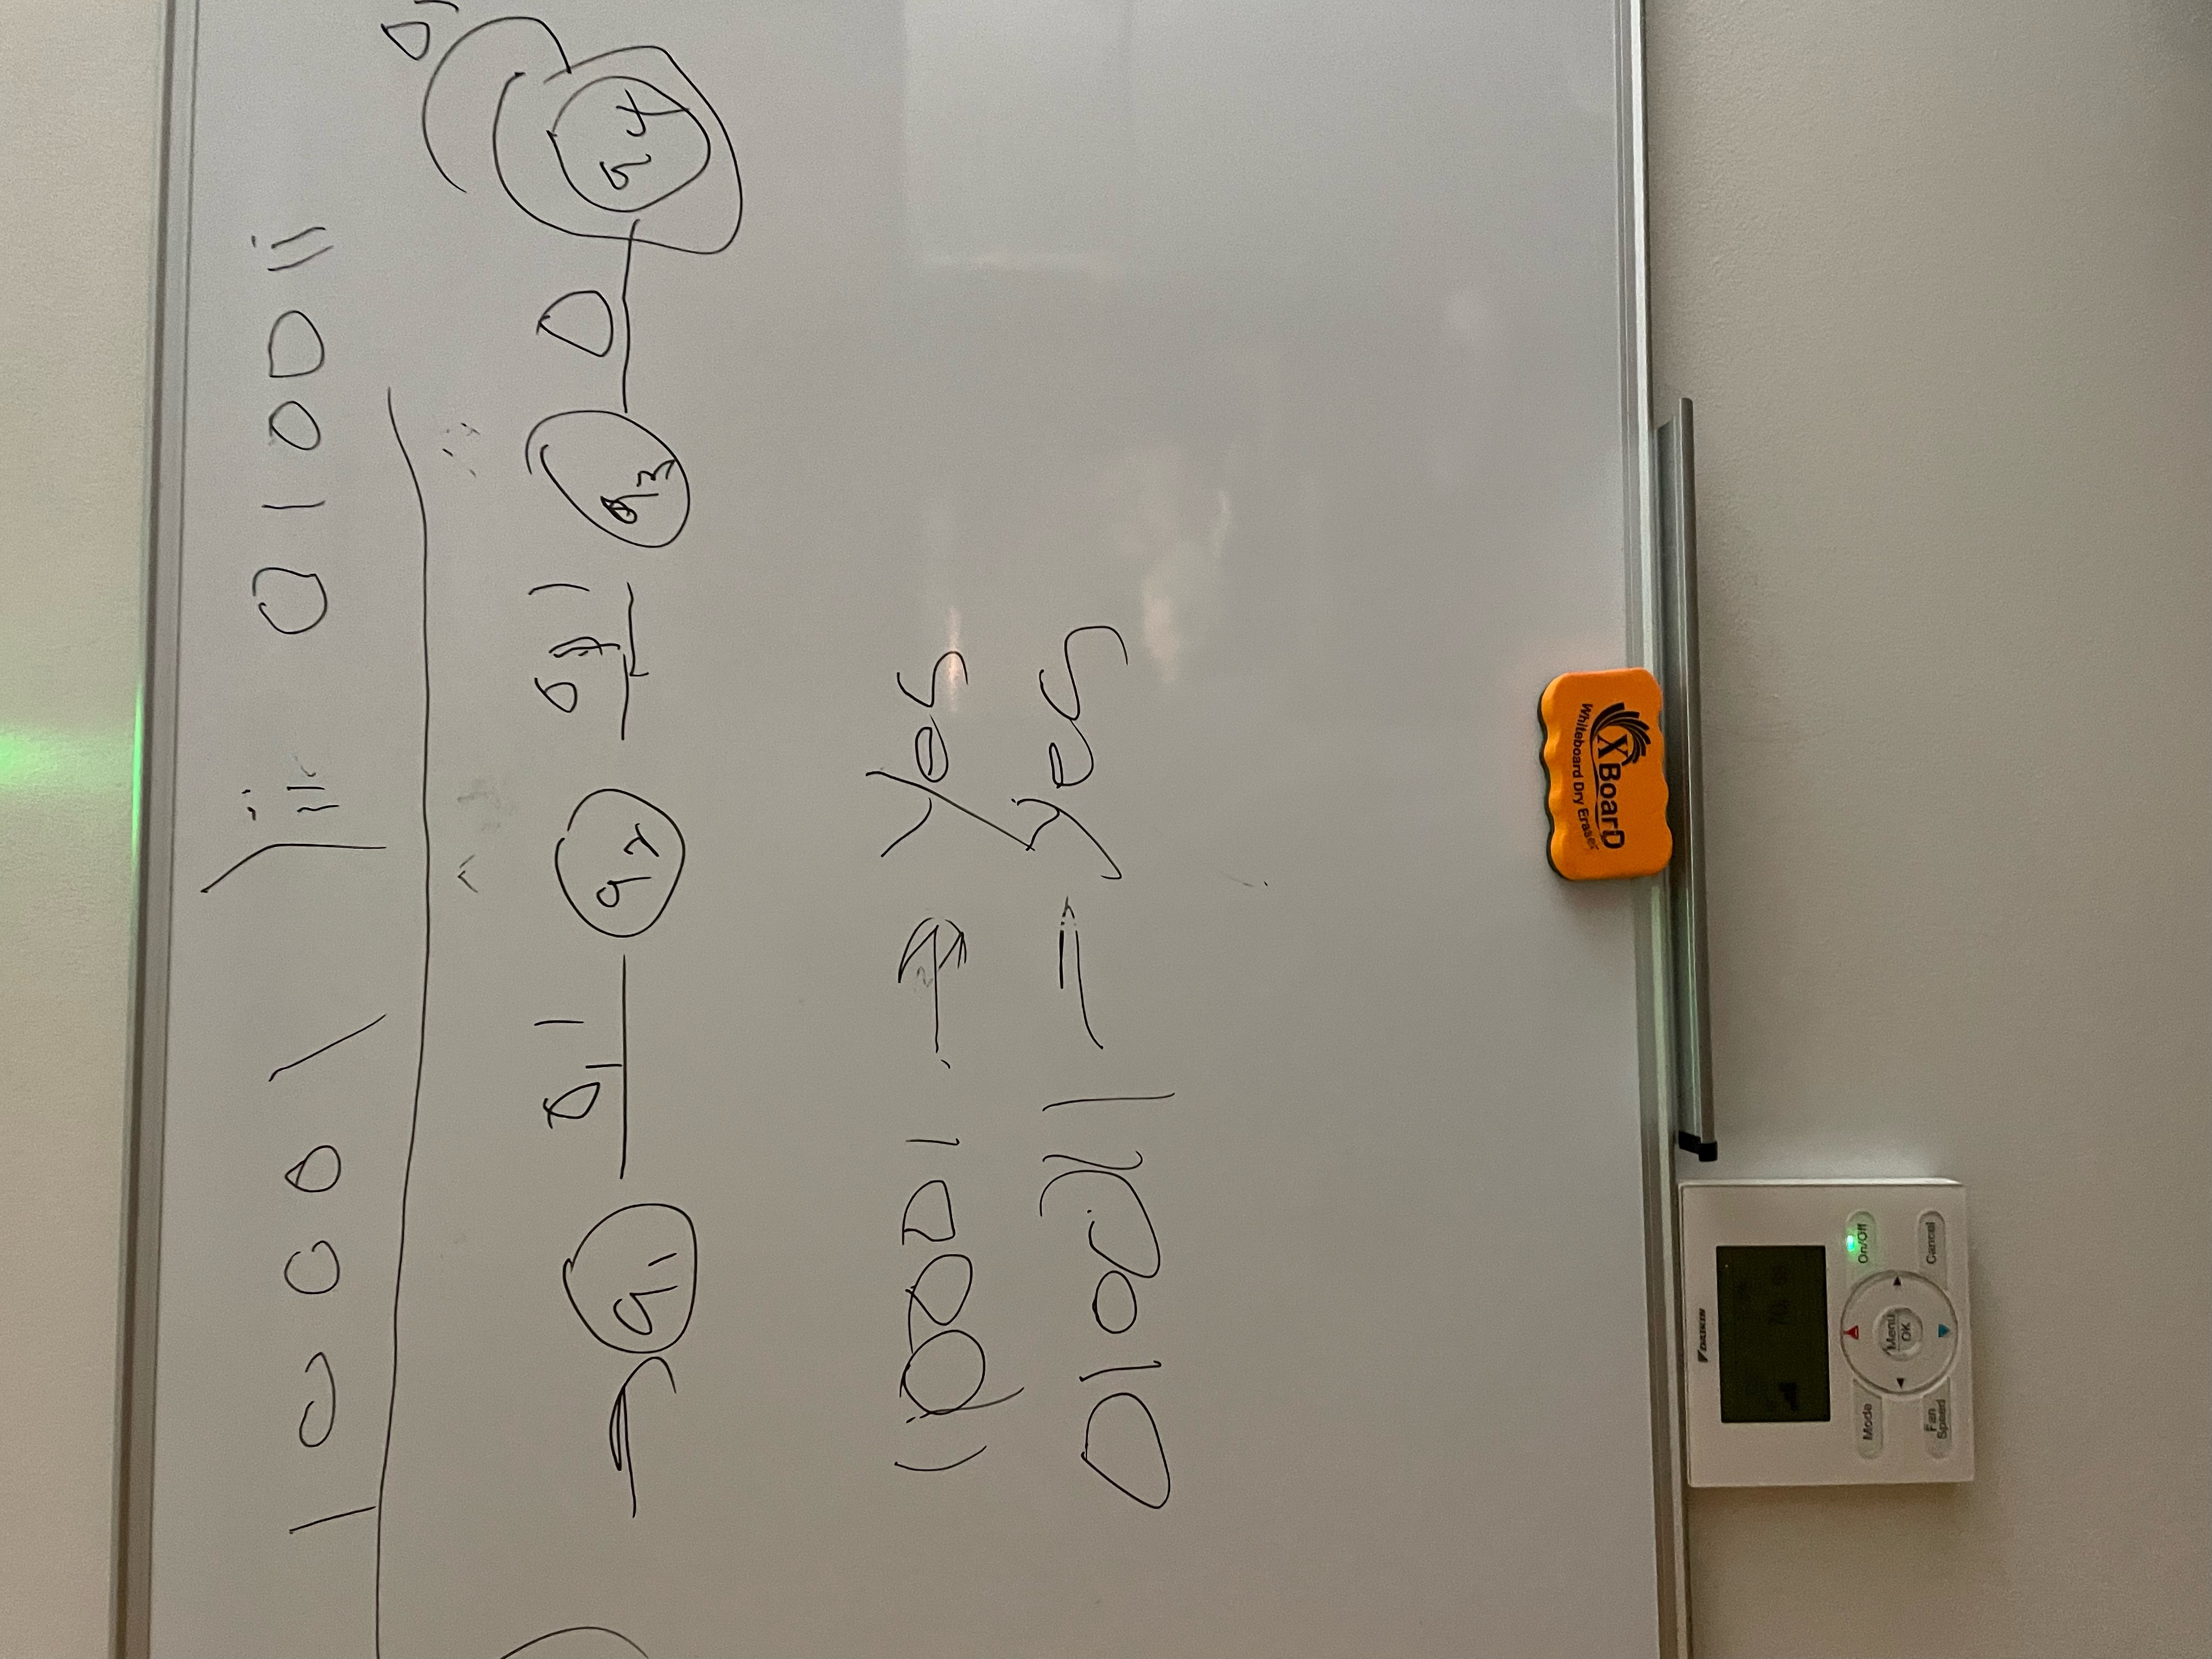
\includegraphics{DFA-b.jpeg}
     \end{center}     
     \item {w $|$ w contains the substring 101} [4 pts] \\
     \begin{center}
          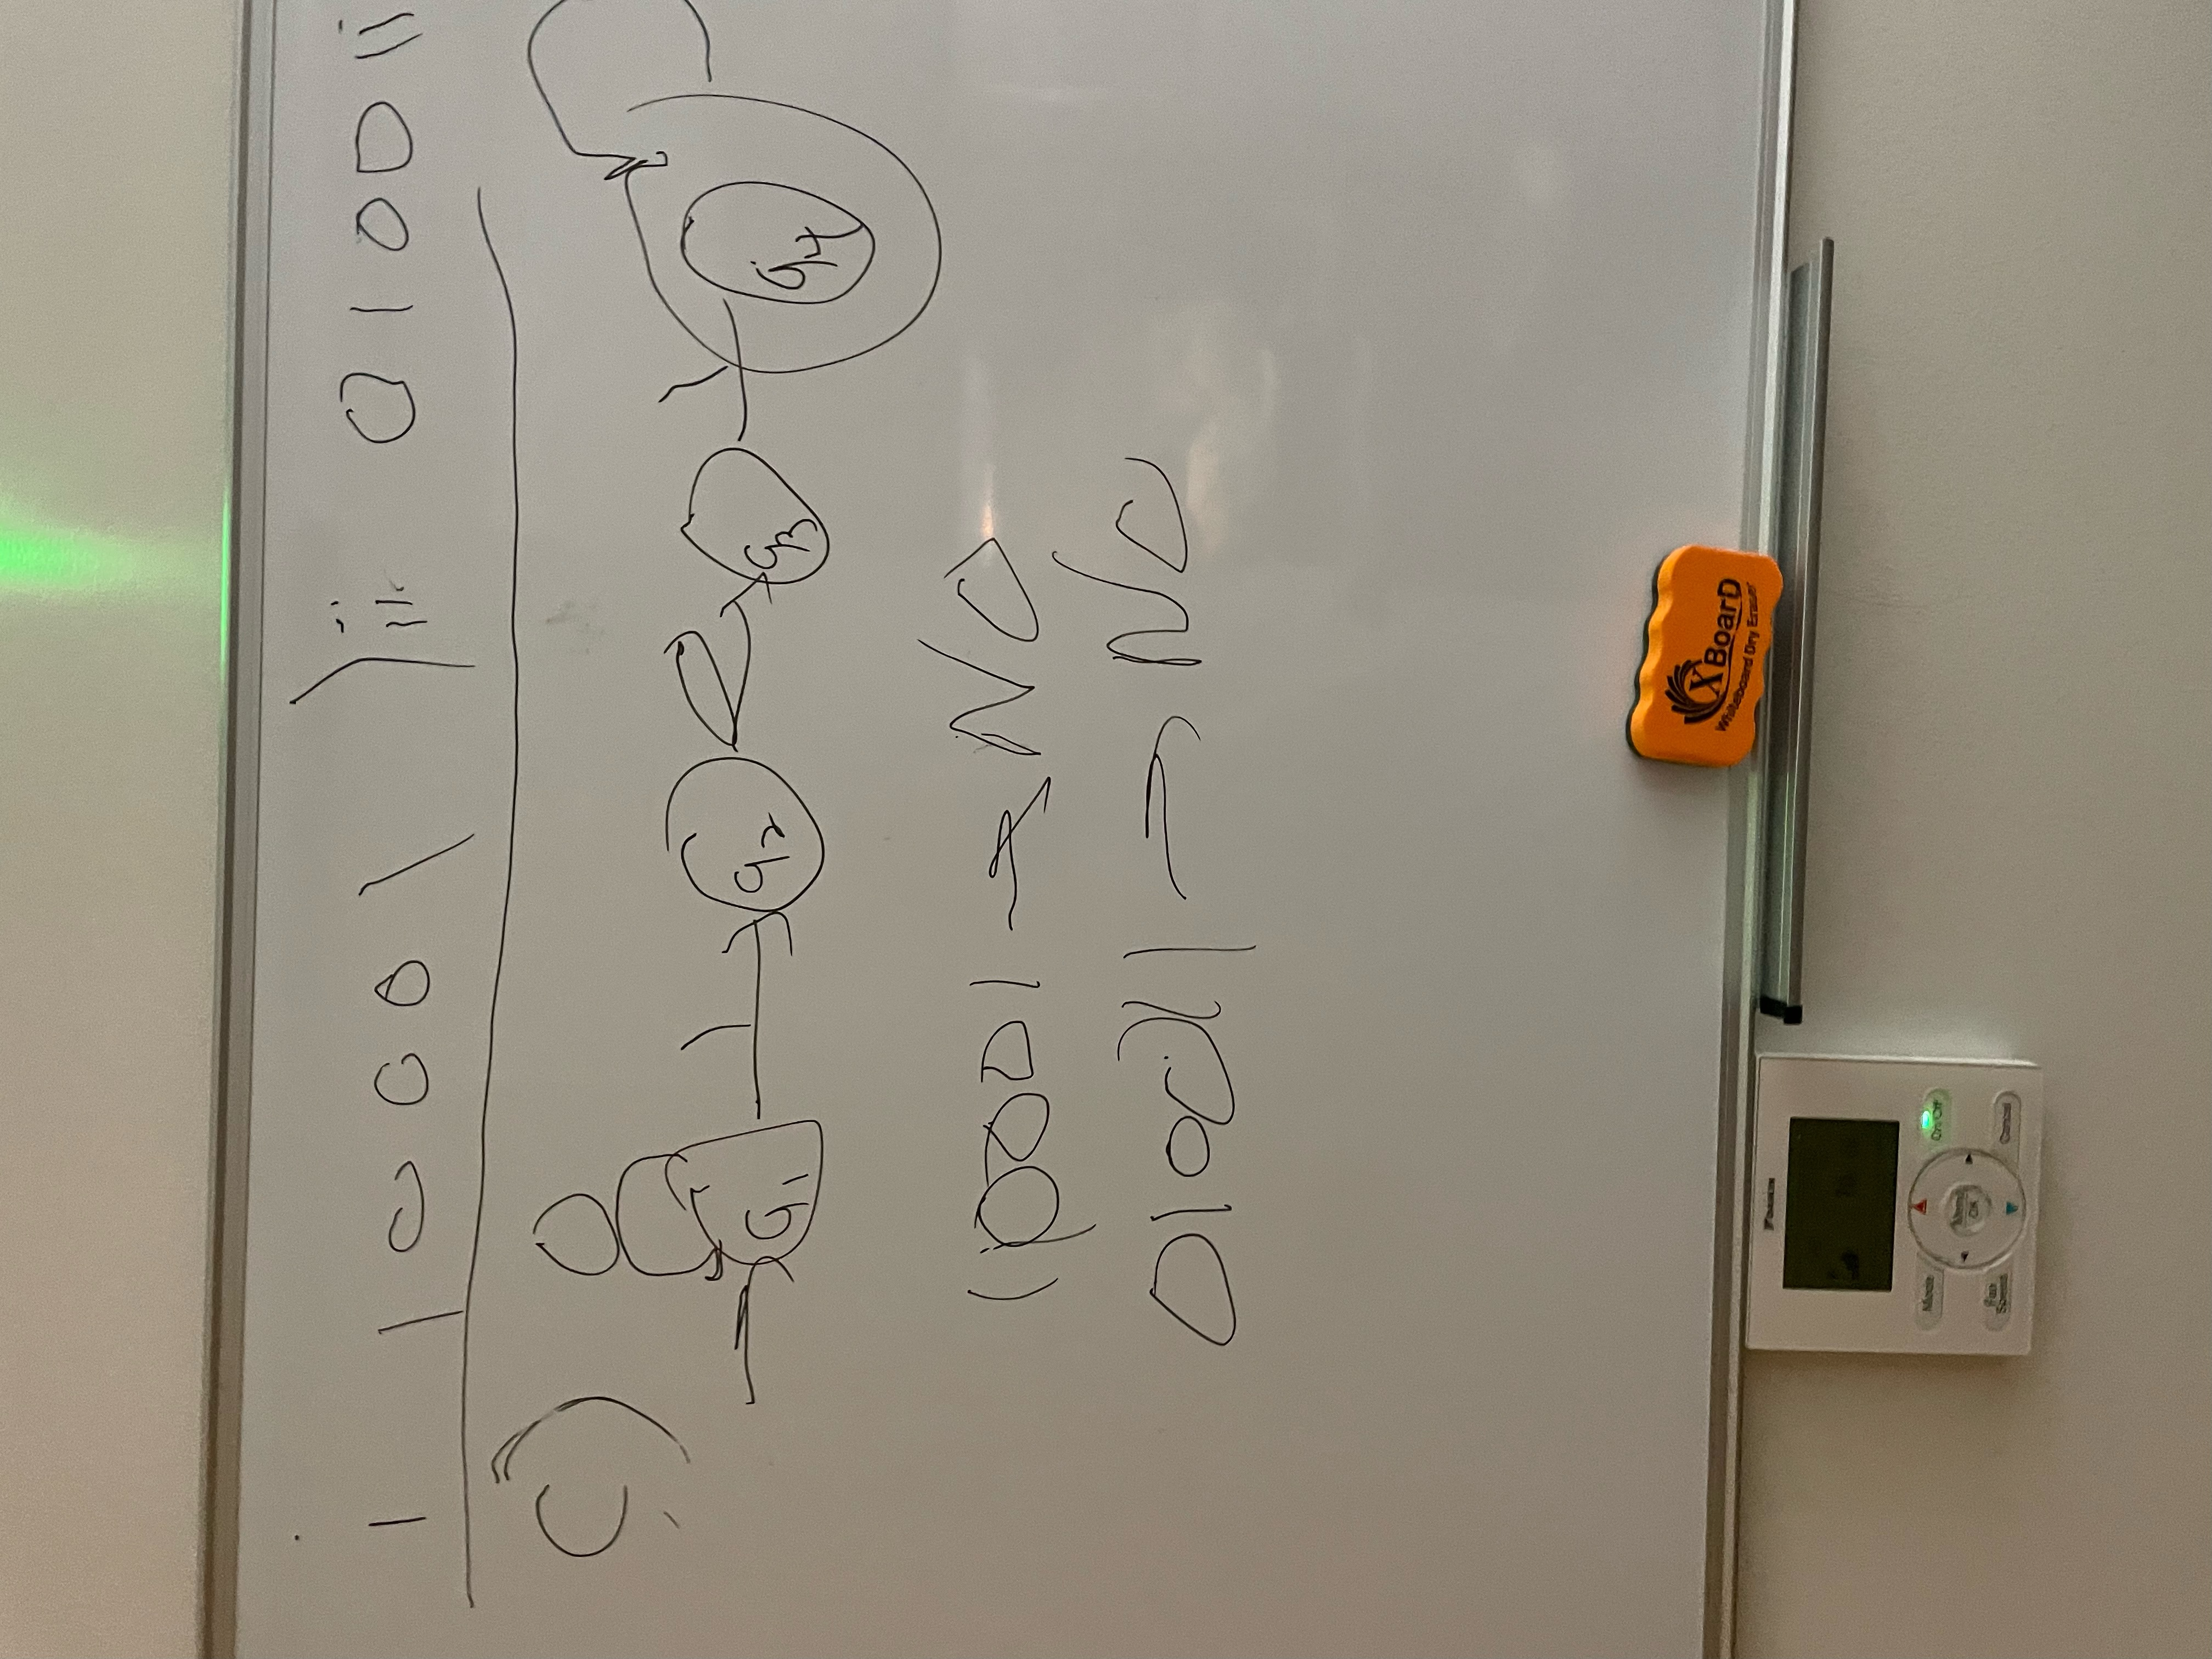
\includegraphics{DFA-c.jpeg}
     \end{center}
     \item {w $|$ w has length at least three and the third symbol is 0} [4 pts] \\
     \begin{center}
          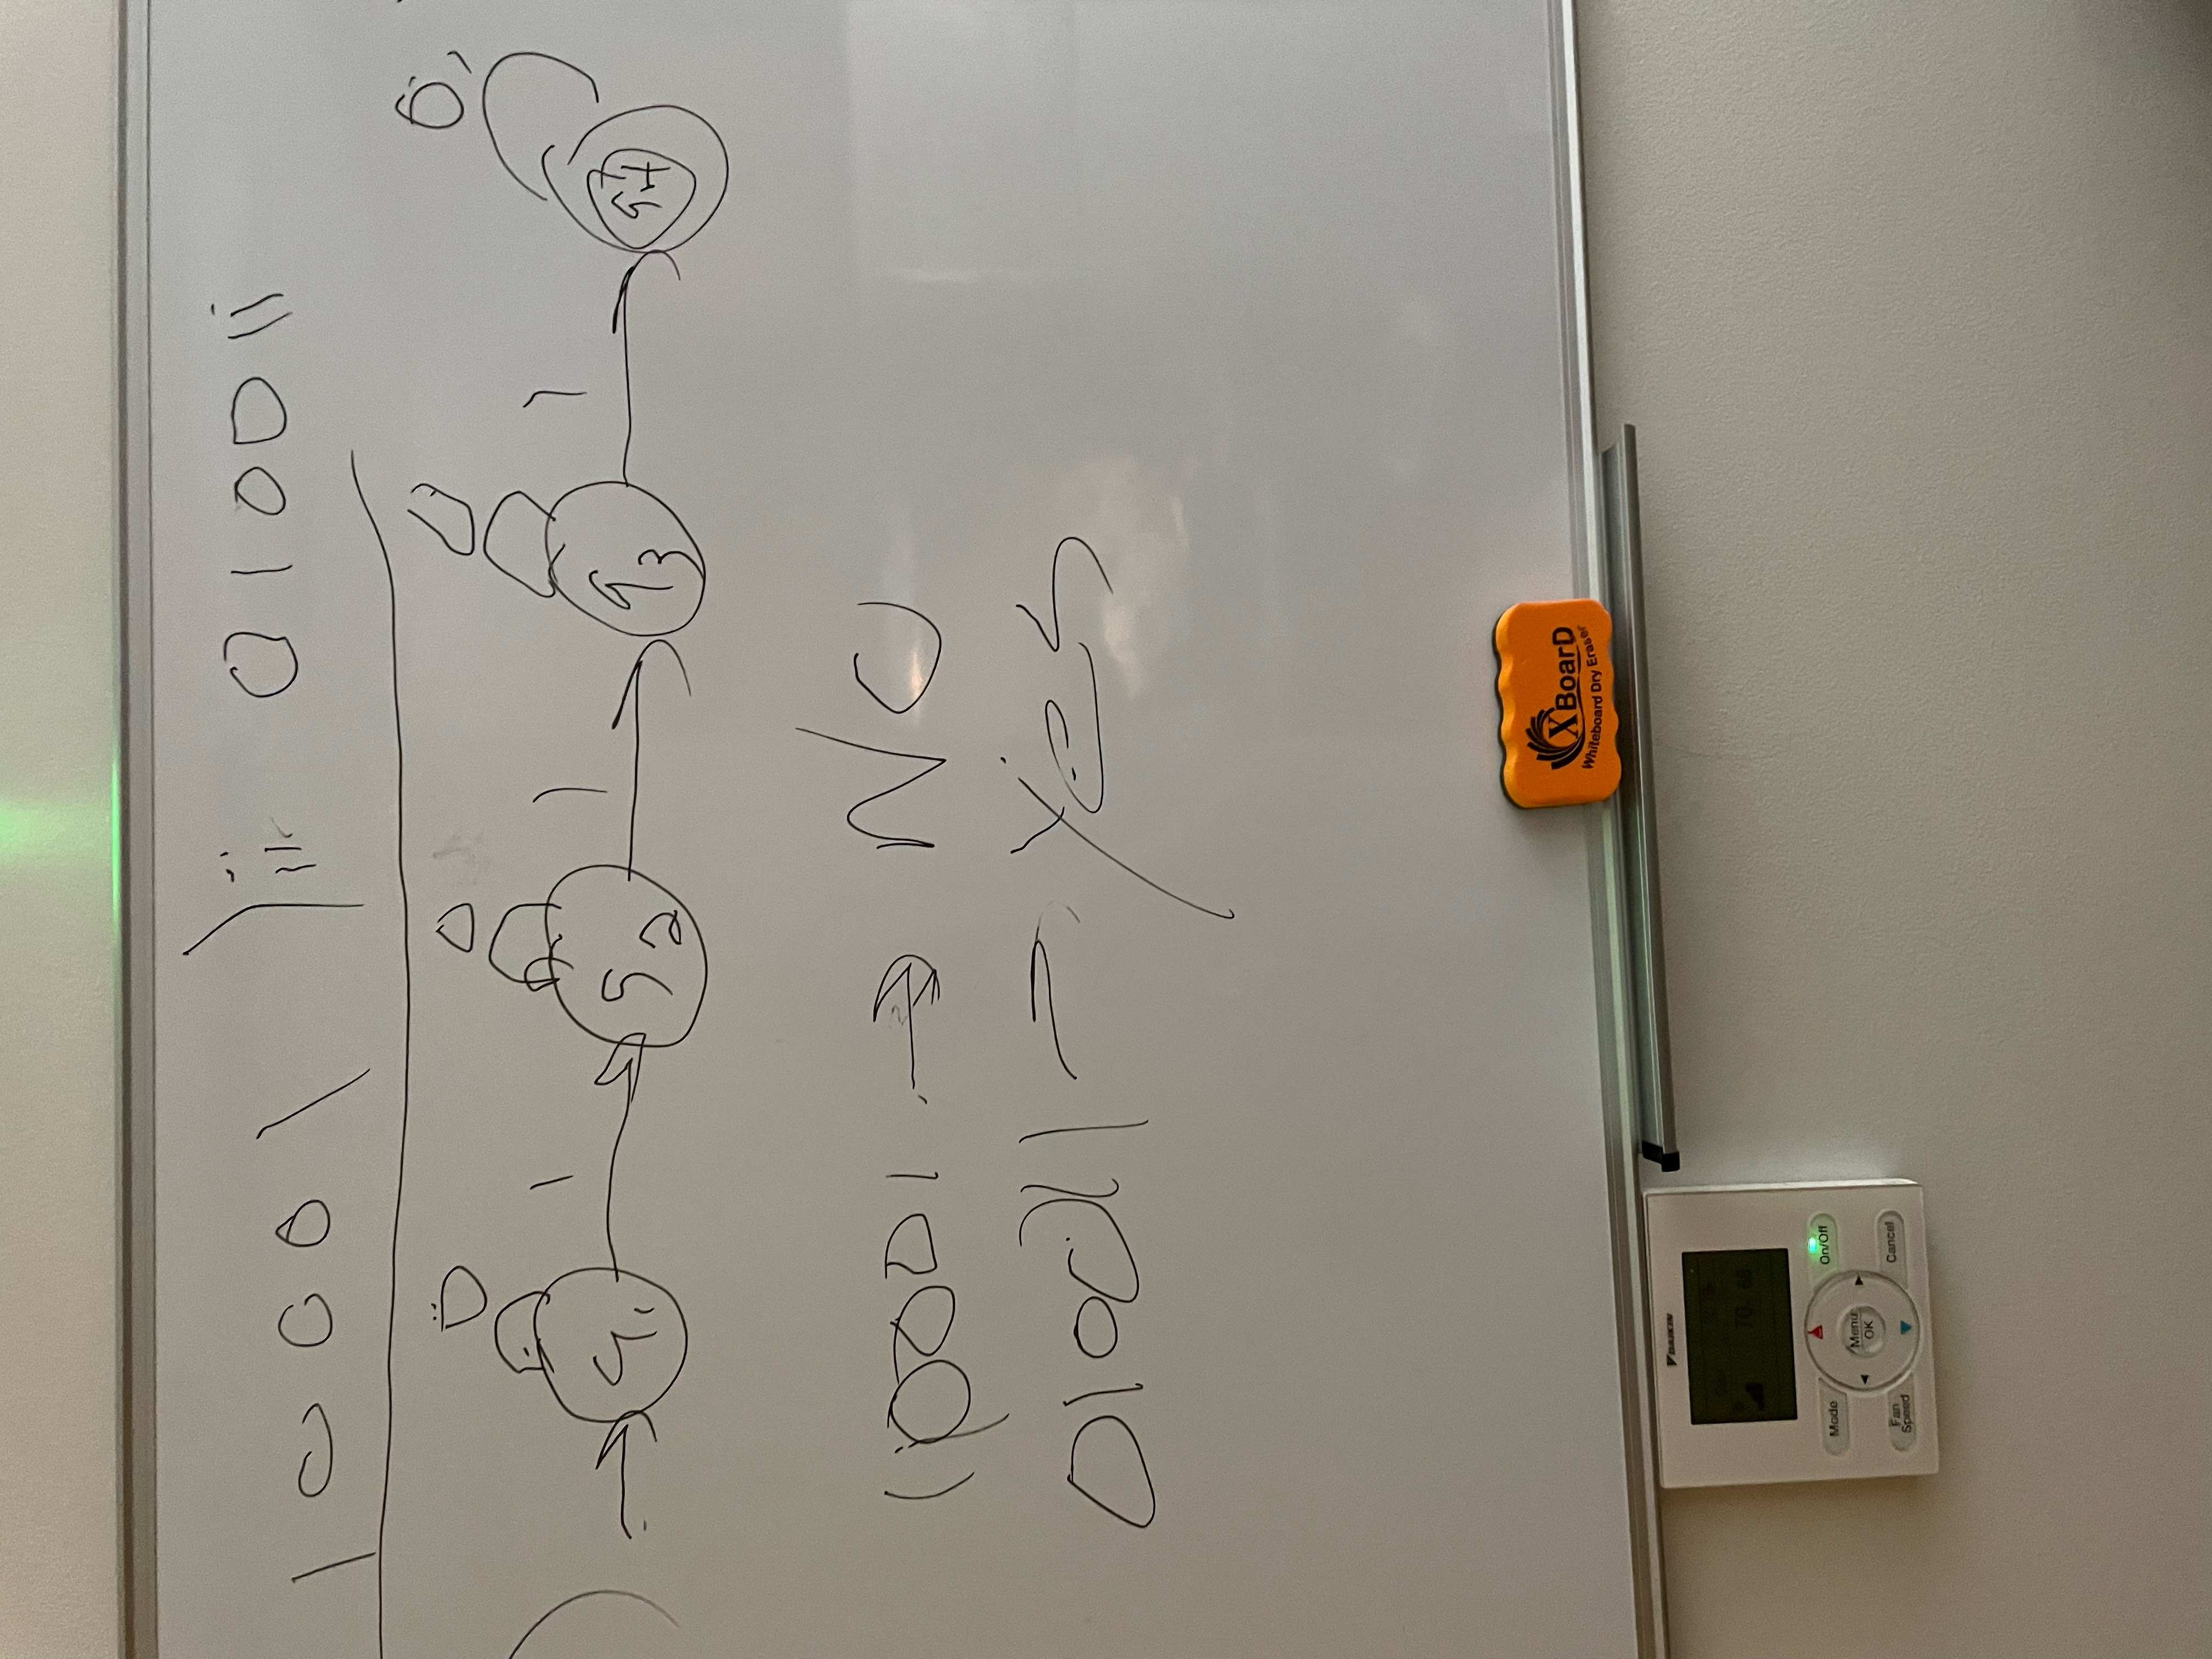
\includegraphics{DFA-d.jpeg}
     \end{center}
     \item {w $|$ the length of w is at most 5} [4 pts] \\
     \begin{center}
          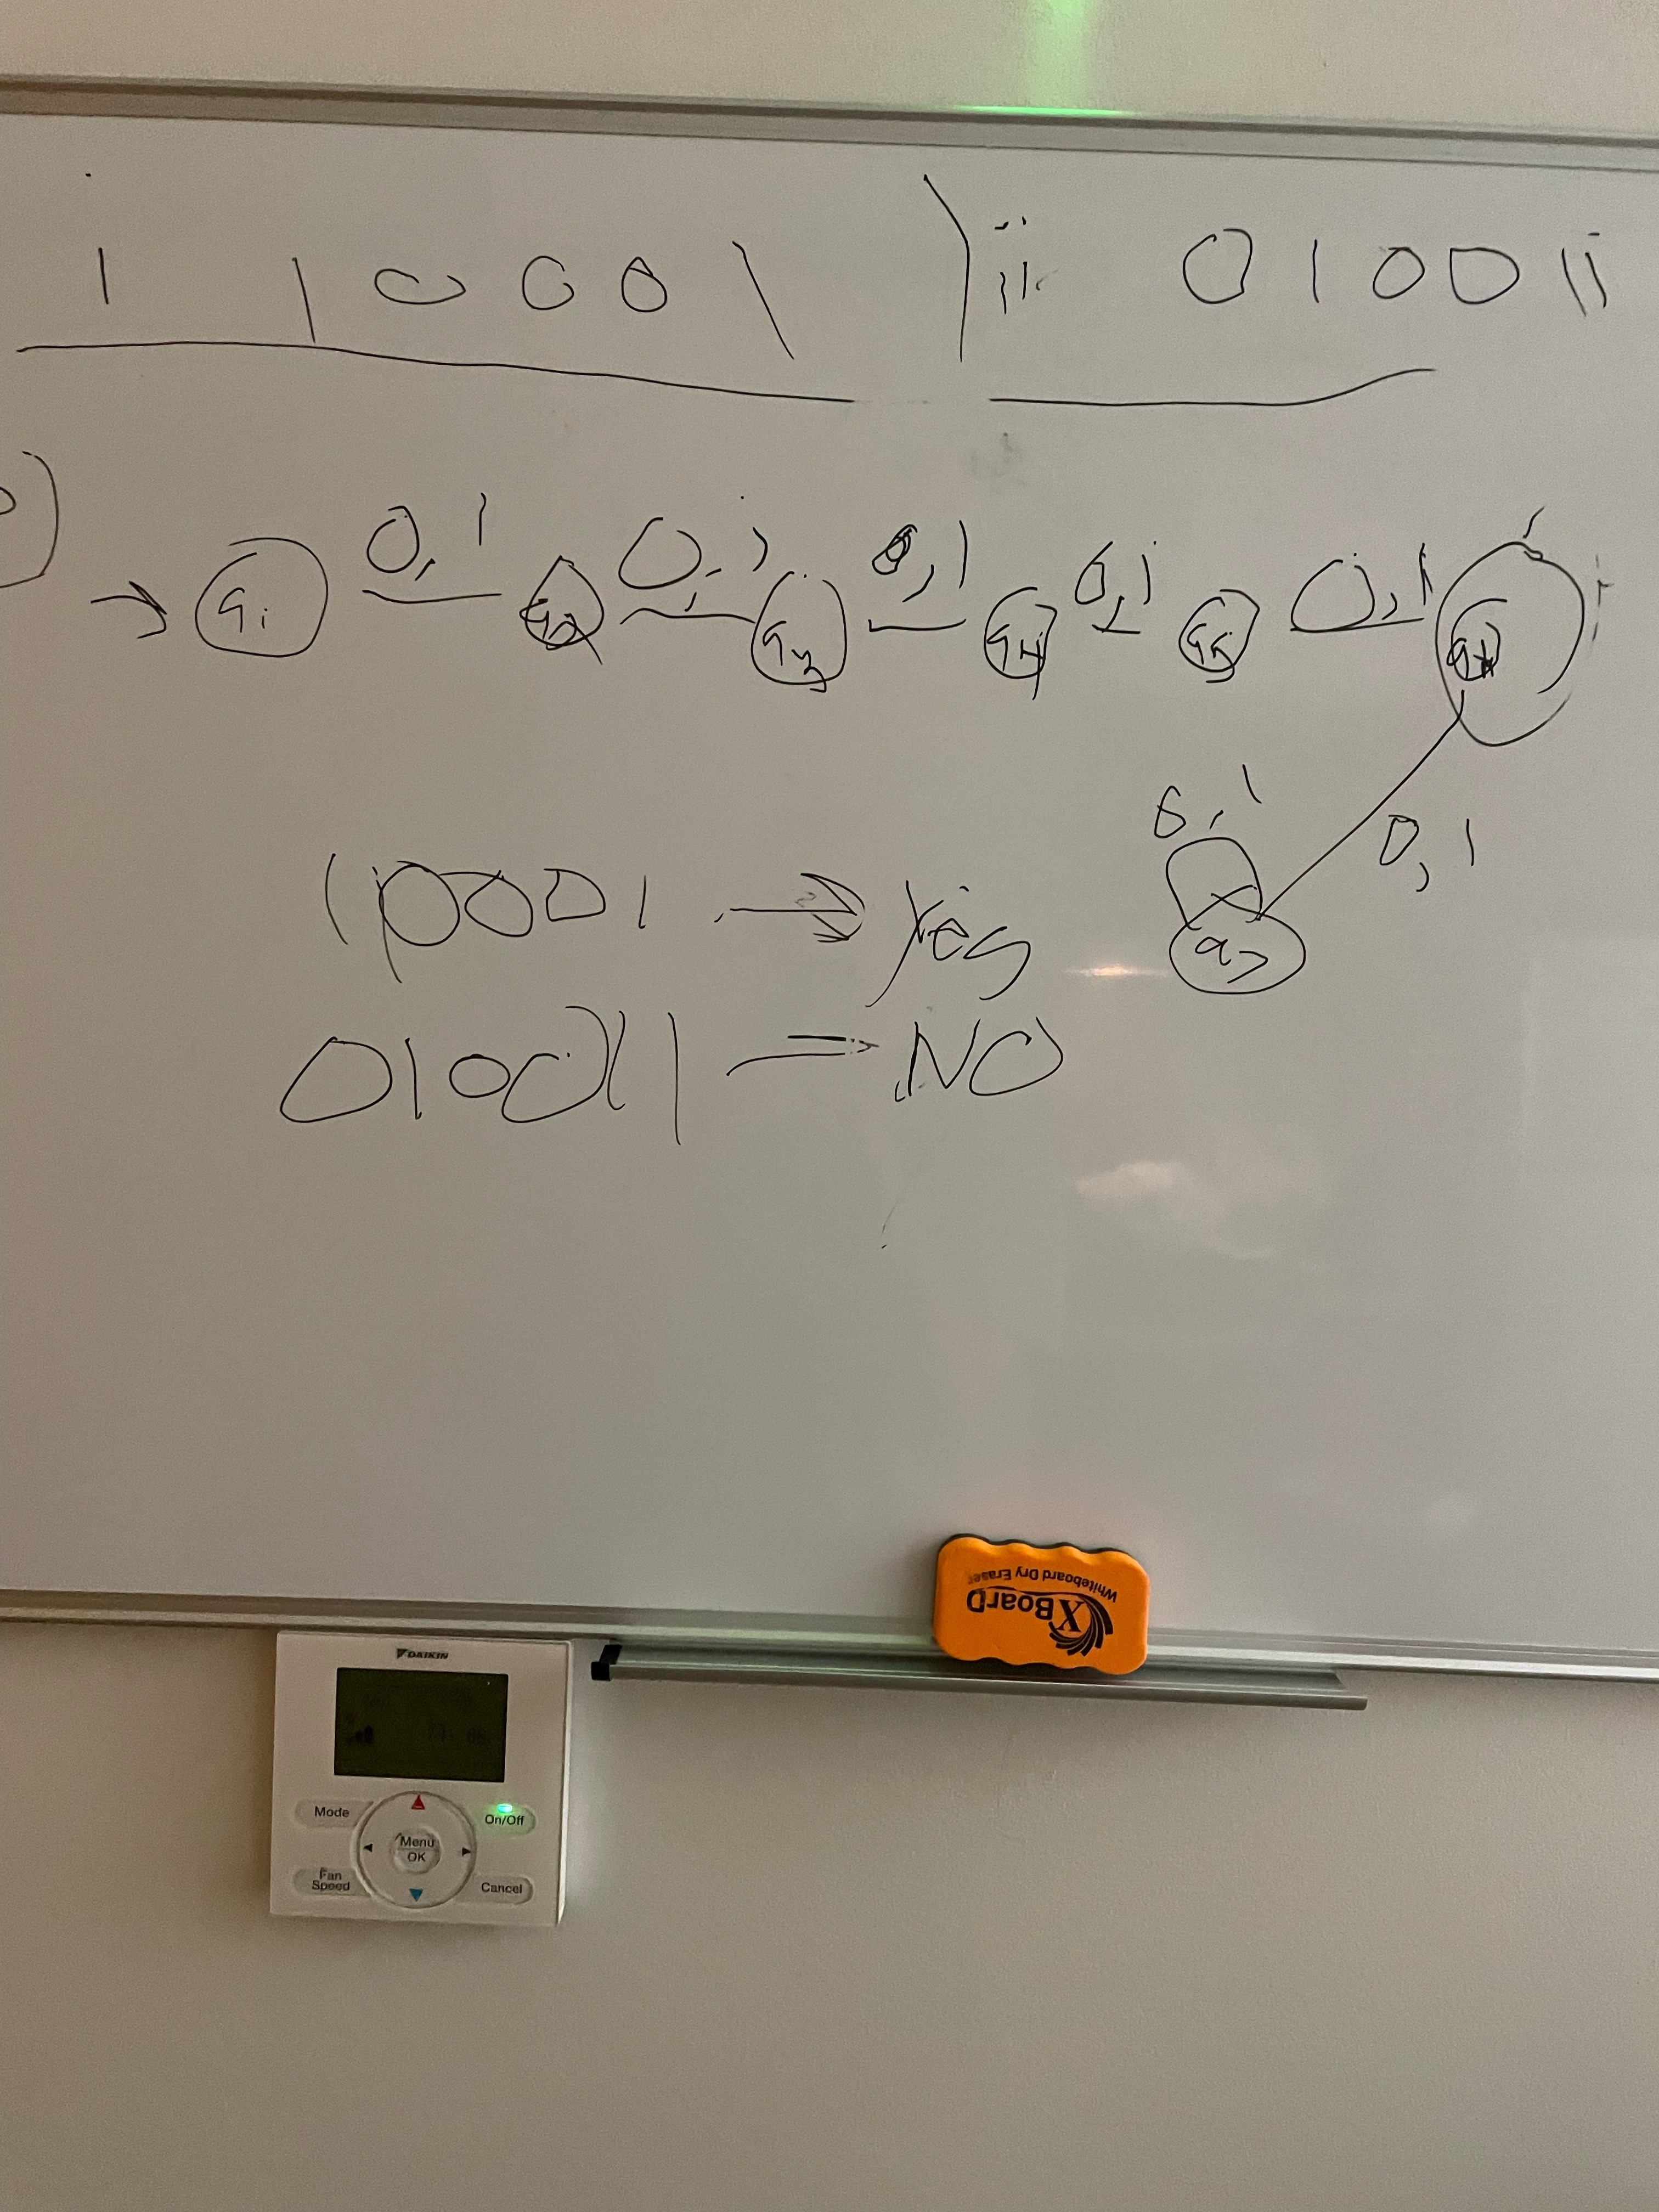
\includegraphics{DFA-e.jpeg}
     \end{center}
   \end{enumerate}
   \item Consider the alphabet $\sigma$ = 1, 2, 3. Write down the members of the set $\sum$ ^2. [2 pts] 
 
   \begin{center}
   	   Answer: $\sum^2$ =\{11,12, 13, 21, 22, 23, 31, 32, 33\}\\
   \end{center}
   
   \item A finite automaton is a 5-tuple (Q, $\sum$ ,$\delta$, q0, F). Consider the finite automaton that recognizes and empty language. Write down F (the set of accepting states ) for this finite automaton.
   
   \begin{center}
   	   Answer: 
   \end{center}
   \item  ”Every deterministic finite autmaton is also a non-deterministic finite automaton”. Justify the statement.
   \begin{center}
   	    Answer: NFA has multiple options for acceptance as well as unable to determine the final state. DFAs are a subset of a possible NFA.
   \end{center}
\end{enumerate}
\end{document}